%% LaTeX-Beamer template for KIT design
%% by Erik Burger, Christian Hammer
%% title picture by Klaus Krogmann
%%
%% version 2.1
%%
%% mostly compatible to KIT corporate design v2.0
%% http://intranet.kit.edu/gestaltungsrichtlinien.php
%%
%% Problems, bugs and comments to
%% burger@kit.edu

\documentclass[18pt]{beamer}

\usepackage[utf8]{inputenc}
\usepackage[babel,german=quotes]{csquotes}
\usepackage{graphicx}
\usepackage{caption}
\usepackage{subfig}
\usepackage[right]{eurosym}
\usepackage{listings}


\usepackage{amssymb} % for |N
\newcommand{\Hilight}{\makebox[0pt][l]{\color{cyan}\rule[-4pt]{0.65\linewidth}{14pt}}}	%from http://newsgroups.derkeiler.com/Archive/Comp/comp.text.tex/2008-10/msg00877.html
\lstset{tabsize=3}

\newcommand{\refframe}
{
	\usebackgroundtemplate
	{
		\begin{pgfpicture}{0mm}{0mm}{\paperwidth}{\paperheight}
		
			\pgfsetnonzerorule
			
			% draw bg color
			{
				\color{black!15}
				\pgfpathrectangle{\pgfpoint{0mm}{0mm}}{\pgfpoint{\paperwidth}{\paperheight}}
				\pgfusepath{fill}
			}
			
			%+ draw grey frame
			{
				\pgfsetcornersarced{\pgfpoint{2mm}{2mm}}
				
				\pgfpathmoveto{\pgfpoint{\paperwidth-1mm}{9mm}}
				\pgfpathlineto{\pgfpoint{1mm}{9mm}}
				\pgfpathlineto{\pgfpoint{1mm}{\paperheight-1mm}}
			}

			{
				\pgfsetcornersarced{\pgfpoint{2mm}{2mm}}
				\pgfpathmoveto{\pgfpoint{1mm}{\paperheight-1mm}}
				\pgfpathlineto{\pgfpoint{\paperwidth-1mm}{\paperheight-1mm}}
				\pgfpathlineto{\pgfpoint{\paperwidth-1mm}{9mm}}
			}
			%- draw grey frame

			\color{yellow}
			\pgfusepath{fill}

		\end{pgfpicture}
	}
}



\author{Robert Schneider, Sven Brauch}


\institute{}

\begin{document}

% change the following line to "ngerman" for German style date and logos
\selectlanguage{ngerman}

\AtBeginSection[]{%
	\begin{frame}
		\tableofcontents[sectionstyle=show/hide,subsectionstyle=hide/show/hide]
	\end{frame}
	\addtocounter{framenumber}{-1}% If you don't want them to affect the slide number
}

%title page
\begin{frame}
\titlepage
\end{frame}

%table of contents
\begin{frame}{Gliederung}
\tableofcontents
\end{frame}


\section{Objektorientierte Programmierung}
\begin{frame}
    \frametitle{Structures}
    \begin{block}{structs}
    Ein \texttt{struct} ist eine Zusammenfassung mehrerer Objekte zu einem größeren.
    Zum Beispiel könnte man ein \texttt{struct} "`Quader"' erstellen, welches drei Fließkommazahlen beinhaltet.
    \end{block}
    \begin{block}{Instanzen}
    Eine solche \texttt{struct} ist lediglich eine abstrakte Beschreibung des Objekts; man arbeitet schließlich mit sogenannten \emph{Instanzen} des Objekts. Beispiel Quader: Die Structure an sich beschreibt das abstrakte Objekt, die Instanz einen konkreten Quader ("`der Quader auf meinem Tisch"').
    \end{block}
\end{frame}
\begin{frame}
    \frametitle{Beispiel für eine Structure}
    \vspace{0.7cm}
    \includegraphics[width=15cm]{example_code/box.pdf}
\end{frame}

\begin{frame}
    \frametitle{Klassen}
    \begin{block}{Klassen}
    Eine \texttt{class} ist eine \texttt{struct}, die zusätzlich zu Daten noch Funktionen enthält, die auf diesen Daten operieren.
    \end{block}
    \begin{block}{Konstruktor und Destruktor}
    Eine Klasse hat zwei besondere Funktionen, den Konstruktor und den Destruktor; der Konstruktor wird aufgerufen, wenn eine neue Instanz der Klasse erstellt wird, und der Destruktor, wenn die Instanz wieder gelöscht wird. Der Konstruktor heißt \texttt{klassenname}, der Destruktor \texttt{\~{}klassenname}.
    \end{block}
\end{frame}
\begin{frame}
    \frametitle{Beispiel für eine Klasse}
    \vspace{0.7cm}
    \includegraphics[width=8.7cm]{example_code/box2.pdf}
\end{frame}
\begin{frame}
    \frametitle{Etwas anderes Beispiel für eine Klasse}
    \includegraphics[width=10.0cm]{example_code/box3.pdf}
\end{frame}


%%%%%%%%%%%%%%%%%%%%%%%%%
% ADD OWN SECTIONS HERE %
%%%%%%%%%%%%%%%%%%%%%%%%%
\section{C++}


\begin{frame}{Was ist C++?}
	\begin{block}{Eine standardisierte Programmiersprache}
		C++
		\begin{itemize}
			\item ist eine Programmiersprache (gibt einen Programmablauf vor)
			\item vereint sowohl high-level- wir auch low-level-Features
			\item ist sehr hardwarenah
			\item ist standardisiert (\emph{hier:} ISO/IEC 14882:2003)
		\end{itemize}
	\end{block}
	
	\pause
	
	\begin{block}{Was sagt der Standard hierzu?}
		C++ is a general purpose programming language based on the C programming language as described in
		ISO/IEC 9899:1990 Programming languages – C.
	\end{block}
\end{frame}

\begin{frame}{Worum geht es bei C++?}
	von-Neumann-Architektur $\xrightarrow{Abstraktion}$ C++ $\xrightarrow{Implementierung}$ Hardware
	
	\begin{itemize}
		\item C++ wurde explizit für die von-Neumann-Architektur designed
		\item C++ soll zero-overhead sein (Features, die ich nicht nutze, benötigen weder Speicher noch Laufzeit)
		\item C++ ist eine Multi-Paradigmen-Sprache mit Betonung der Objektorientierung
	\end{itemize}
	
	\begin{block}{Standard, 1.8}
		The constructs in a C++ program create, destroy, refer to, access, and manipulate objects.
	\end{block}
\end{frame}

\begin{frame}{Wofür nutze ich C++?}
	foo!
\end{frame}

\begin{frame}[fragile]{»Dinge«}
	Das grundlegende Konzept in C++ nennt sich im Standard \enquote{object}. Hinsichtlich Java und Objektorientierung aber missverständlich!
	Wir nennen es daher »Ding«.
	
	\pause
	
	\small
	\begin{block}{Standard, 1.8}
		Ein »Ding«
		\begin{itemize}
			\item ist ein Speicherbereich, aber \emph{keine} Funktion (auch wenn diese Speicher belegt!).
			\item wird durch eine Definition, den \verb|new|-Ausdruck oder vom Compiler erzeugt.
			\item hat einen Typen und eine Speicherdauer {\tiny (die die Lebensdauer des dort gespeicherten »Objekts« beeinflusst)}; \emph{kann} einen \emph{Namen} haben.
			\item hat eine Größe von einem oder mehr Bytes {\tiny (abgesehen von bit-fields)}.
			\item von »einfachem« {\tiny (POD)} Typ besetzt eine zusammenhängende Menge Bytes.
		\end{itemize}
	\end{block}
\end{frame}

\begin{frame}[fragile]{Speicher}
	\begin{block}{Standard, 1.7}
		Die fundamentale Speicher-Einheit im C++ Speichermodell ist das \emph{Byte}. [Es folgt eine sehr abstrakte Definition.]
		Der Speicher, welcher einem C++ Programm zur Verfügung steht, besteht aus einer oder mehreren Sequenzen von zusammenhängenden Bytes.
		Jedes Byte hat eine eindeutige Adresse.
	\end{block}
	
	\footnotesize
	\begin{block}{}
		\begin{lstlisting}[language=C++]
			int foo;
			int bar;
			double d;
			double& rd = d;
			
			cout << sizeof(foo);
			cout << sizeof(int);
		\end{lstlisting}
	\end{block}
\end{frame}

%, memory model, object model, Ring HW-Standard-Impl
\section{»Dinge«, Referenzen und Pointer}


\subsection{»Dinge« und Speicher}

\begin{frame}[fragile]{»Dinge«}
	Das grundlegende Konzept in C++ nennt sich im Standard \enquote{object}. Hinsichtlich Java und Objektorientierung aber missverständlich!
	Wir nennen es daher »Ding«.
	
	\pause
	
	\begin{block}{Standard, 1.8}
		Ein »Ding«
		\begin{enumerate}
			\item ist ein Speicherbereich, aber \emph{keine} Funktion {\tiny(auch wenn diese Speicher belegt!)}.
			\item hat eine Speicherdauer, einen Typen und \emph{kann} einen \emph{Namen} haben.
			\item {\scriptsize hat eine Größe von einem oder mehr Bytes {\tiny (abgesehen von bit-fields)}.}
			\item {\scriptsize von »einfachem« {\tiny (POD)} Typ besetzt eine zusammenhängende Menge Bytes.}
			\item {\scriptsize wird durch eine Definition, den \verb|new|-Ausdruck oder vom Compiler erzeugt.}
		\end{enumerate}
	\end{block}
\end{frame}

\begin{frame}[fragile]{Speicher}
	\begin{block}{Standard, 1.7}
		Die fundamentale Speicher-Einheit im C++ Speichermodell ist das \emph{Byte}. [Es folgt eine sehr abstrakte Definition.]
		Der Speicher, welcher einem C++ Programm zur Verfügung steht, besteht aus einer oder mehreren Sequenzen von zusammenhängenden Bytes.
		Jedes Byte hat eine eindeutige Adresse.
	\end{block}
	
	\pause
	
	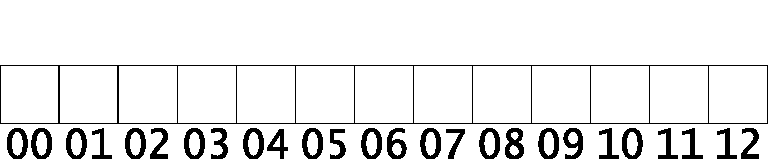
\includegraphics[width=\linewidth]{images/free}
\end{frame}

\begin{frame}[fragile]{»Dinge« und Speicher}
	Alle Definitionen legen »Dinge« an.\\
	{\tiny Ausnahme: \verb|static|}
	
	{\footnotesize
	\begin{block}{}
		\lstinputlisting[language=C++, linerange={3-4, 6-6}]{cpp-code/objects.cpp}
	\end{block}
	}
	
	\pause
	\vspace{1em}
	
	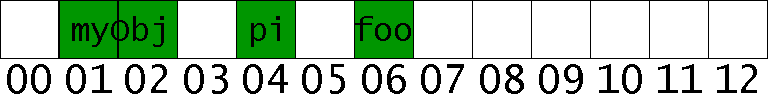
\includegraphics[width=\linewidth]{images/object_things}
\end{frame}


\subsection{Referenzen}

\begin{frame}[fragile]{Referenz: Referenzen}
	\verb|TYPE& add\_name = orig\_name;|
	\begin{itemize}
		\item Führt \verb|add_name| als zusätzlichen Namen für das »Ding« mit dem Namen \verb|orig_name| ein.
		\item \verb|add_name| heißt auch eine Referenz auf \verb|orig_name|.
	\end{itemize}
	
	\vspace{2em}
	
	Achtung: Eine Referenz muss immer gleich »initialisiert« werden, d.h. mittels \verb|=| einem »Ding« zugeordnet. {\tiny Bei Klassen-Membern in der Initialisations-Liste des Konstruktors.}
\end{frame}

\begin{frame}[fragile]{»Dinge« und Referenzen}
	Eine Referenz ist ein zusätzlicher Namen für \emph{dasselbe} »Ding«.\\
	Die Speicherdauer wird dadurch \emph{nicht} beeinflusst.
	
	{\footnotesize
	\begin{block}{}
		\lstinputlisting[language=C++, linerange=14-15]{cpp-code/objects.cpp}
	\end{block}
	}
	
	\pause
	
	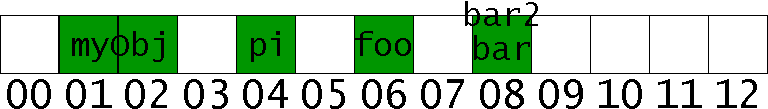
\includegraphics[width=\linewidth]{images/object_refs}
	
	\pause
	
	{\footnotesize
	\begin{block}{}
		\lstinputlisting[language=C++, linerange=16-17]{cpp-code/objects.cpp}
	\end{block}
	}
\end{frame}

\begin{frame}[fragile]{Referenzen als Parameter}
	Nutzt man eine Referenz als Parameter, so kann man innerhalb der Funktion den Wert des übergebenen »Dings« ändern:
	
	{\footnotesize
	\begin{block}{}
		\lstinputlisting[language=C++, linerange=34-38]{cpp-code/objects.cpp}
	\end{block}
	}
	
	\pause
	
	{\footnotesize
	\begin{block}{}
		\lstinputlisting[language=C++, linerange=19-22]{cpp-code/objects.cpp}
	\end{block}
	}
\end{frame}


\subsection{Pointer}

\begin{frame}[fragile]{Adressen und Pointer}
	Jedes Byte hat eine eindeutige Adresse.
	
	Man darf keine Annahmen darüber treffen, wie diese Adresse tatsächlich aussieht oder wie groß sie ist!
	Was man tun darf, sind Operationen mit \emph{Pointern}. Pointer sind Container von Adressen.
	
	\pause
	\vspace{1em}
	
	Wir wollen jedoch zwecks Anschauung eine Adresse mit der Nummer \emph{der} Bytes eines »Dings« identifizieren.
	
	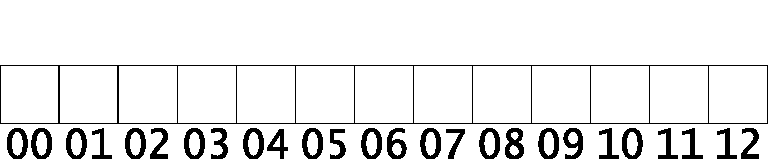
\includegraphics[width=\linewidth]{images/free}
\end{frame}

\begin{frame}[fragile]{»Dinge« und Pointer}
	Sei \verb|NAME| der Name eines »Dings«. Mit \verb|&NAME| erhalte ich dann die Adresse des »Dings«. Die Adresse selbst ist auch wieder ein »Ding«!
	
	\vspace{1em}
	\pause
	
	Als »Ding« hat die Adresse einen Typ:
	{\footnotesize
	\begin{block}{}
		\lstinputlisting[language=C++, linerange=24-25]{cpp-code/objects.cpp}
	\end{block}
	}
	
	\pause
	
	Das »Ding« \verb|NAME| habe den Typen \verb|TYPE|. Dann hat die Adresse des »Dings« den Typ \verb|TYPE*|.
\end{frame}


\begin{frame}[fragile]{»Dinge«, Pointer und Adressen}
	Ein Beispiel:
	
	{\footnotesize
	\begin{block}{}
		\lstinputlisting[language=C++, linerange={3-4, 6-6}]{cpp-code/objects.cpp}
	\end{block}
	}
	
	\vspace{1em}
	\phantom{
		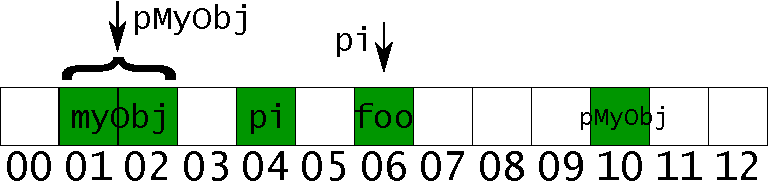
\includegraphics[width=\linewidth]{images/object_points_addr}
	}
\end{frame}

	\begin{frame}[fragile]{»Dinge«, Pointer und Adressen}
		Ein Beispiel:
		
		{\footnotesize
		\begin{block}{}
			\lstinputlisting[language=C++, linerange={3-4, 6-6, 10-10}]{cpp-code/objects.cpp}
		\end{block}
		}
		
		\vspace{1em}
		\phantom{
			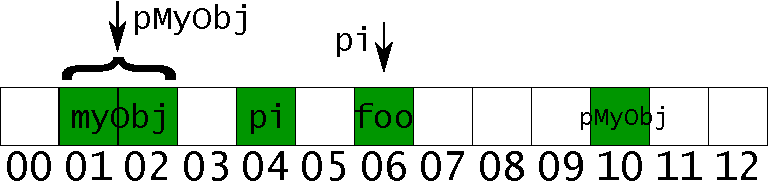
\includegraphics[width=\linewidth]{images/object_points_addr}
		}
	\end{frame}

	\begin{frame}[fragile]{»Dinge«, Pointer und Adressen}
		Ein Beispiel:
		
		{\footnotesize
		\begin{block}{}
			\lstinputlisting[language=C++, linerange={3-4, 6-6, 10-10, 27-27}]{cpp-code/objects.cpp}
		\end{block}
		}
		
		\pause
		\vspace{1em}
		
		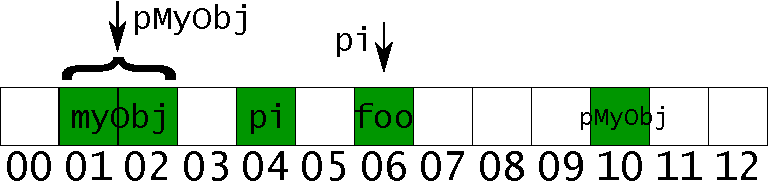
\includegraphics[width=\linewidth]{images/object_points_addr}
	\end{frame}


\begin{frame}[fragile]{Pointer vs. Referenzen}
	\footnotesize
	\begin{tabular}{c|c}
		Pointer & Referenz \\ \hline
		ist ein »Ding« & ist nur ein zusätzlicher Name \\
		enthält eine Adresse & enthält selbst nichts \\
		Inhalt kann sich ändern & bezieht sich immer auf dasselbe »Ding« \\
		Inhalt muss nicht sinnvoll sein & bezieht sich auf ein existierendes »Ding« \\
	\end{tabular}
	
	\pause
	
	{\footnotesize
	\begin{block}{}
		\lstinputlisting[language=C++, linerange={4-4, 27-31}]{cpp-code/objects.cpp}
	\end{block}
	}
\end{frame}


\section{Stack und Heap}
\subsection{Stack}

\newcommand{\stackframe}[3]{
	\begin{frame}[t]{#1}
		\begin{columns}
			\column[t]{0.25\textwidth}
				\ifthenelse{ \equal{#2}{\empty} }{}
				{
					\includegraphics[width=\linewidth]{images/#2}
				}
			
			\column[t]{0.75\textwidth}
				\begin{block}{}
					#3
				\end{block}
		\end{columns}
	\end{frame}
}



\begin{frame}[fragile]{Speicherdauer von »Dingen«}
	\begin{block}{Block}
		\begin{itemize}
			\item Ein \emph{Block} beginnt mit einer \verb|{| und endet mit der nächsten \verb|}|.
			\item {\footnotesize Ein Block kann mehrere \emph{statements} enthalten -- z.B. Definitionen, Zuweisungen, Funktionsaufrufe usw.}
			\item {\footnotesize Anderer Name: \emph{compound statement}}
			\item {\footnotesize Die geschweiften Klammern bezeichnen \emph{keine} Blöcke bei: Klassen, \verb|namespace|, \verb|enum|}
		\end{itemize}
	\end{block}
	
	\pause
	\vspace{1em}
	
	Definiere ich ein »Ding«, so wird es bis zum Ende des Blocks, in welchem es erzeugt wurde, gespeichert.
	
	\vspace{0.5em}
	
	Diese Art der vorgegebenen Speicherdauer nennt sich \emph{automatic storage duration}.
\end{frame}

\begin{frame}[fragile]{Referenz: Definition von »Dingen«, Auf-den-Stack-legen}
	\verb|TYPE name;| \hspace{1em} bzw. \hspace{1em} \verb|TYPE name(PARAMETER);|
	\begin{itemize}
		\item Stellt sicher, dass es Speicher für das »Ding« vom Typ \verb|TYPE| gibt.
		\item Führt den Namen \verb|name| für das »Ding« ein.
		\item Ruft den Konstruktor des »Dings« auf (und übergibt die PARAMETER).
	\end{itemize}
	
	\vspace{1em}
	
	\verb|TYPE name[STATIC_NUMBER];| -- die Variante mit Parametern \emph{existiert nicht!}
	\begin{itemize}
		\item Stellt sicher, dass es Speicher für \verb|STATIC_NUMBER| »Dinge« gibt.
		\item Führt den Namen \verb|name| ein, dieser ist (fast) identisch zur Adresse des nullten Elements.
		\item Ruft nacheinander für jedes Element den \emph{default}-Konstruktor auf, beginnend beim nullten Element.
	\end{itemize}
\end{frame}

\begin{frame}{Reihenfolge der Definitionen}
	\begin{itemize}
		\item Wenn ich (mehrere) »Dinge« innerhalb eines Blocks definiere, werden diese in der Reihenfolge der Definition auf einen Stapel abgelegt -- den \emph{Stack}.
		\item Das ist nicht wörtlich zu nehmen! Der Stack ist nur gedanklich!
		\item Beim Ende des Blocks werden die »Dinge« wieder vom Stack genommen, und zwar in der Reihenfolge, in welcher sie definiert wurden (Standard, 6.6 2).
	\end{itemize}
	
	\pause
	\vspace{1em}
	
	Man kann dieses Verhalten nicht beeinflussen!
\end{frame}

\begin{frame}[fragile]{Referenz: Vom-Stack-nehmen}
	Für ein »Ding«, welches als \verb|TYPE name| definiert wurde:
	\begin{itemize}
		\item Ruft den Destruktor des »Dings« auf.
		\item Gibt den reservierten Speicher wieder frei.
	\end{itemize}
	
	\vspace{2em}
	
	Für ein »Ding«, welches als \verb|TYPE name[STATIC_NUMBER]| definiert wurde:
	\begin{itemize}
		\item Ruft nacheinander für jedes Element den Destruktor auf, beginnend beim nullten Element.
		\item Gibt den reservierten Speicher wieder frei.
	\end{itemize}
\end{frame}


\stackframe{Am Anfang war die Leere\dots}{\empty}{
	\lstinputlisting[language=C++, linerange=1-1]{cpp-code/stack.cpp}
}

\stackframe{Definition von »Dingen« (1)}{stack_1}{
	\lstinputlisting[language=C++, linerange=1-3]{cpp-code/stack.cpp}
}

\stackframe{Definition von »Dingen« (2)}{stack_2}{
	\lstinputlisting[language=C++, linerange=1-4]{cpp-code/stack.cpp}
}

\stackframe{Definition von »Dingen« (3)}{stack_2_plus}{
	\lstinputlisting[language=C++, linerange=1-5]{cpp-code/stack.cpp}
}

\stackframe{Definition von »Dingen« (4)}{stack_3}{
	\lstinputlisting[language=C++, linerange=1-6]{cpp-code/stack.cpp}
}

\stackframe{Definition von »Dingen« (5)}{stack_4}{
	\lstinputlisting[language=C++, linerange=1-7]{cpp-code/stack.cpp}
}

\stackframe{Definition von »Dingen« (6)}{stack_3}{
	\lstinputlisting[language=C++, linerange=1-8]{cpp-code/stack.cpp}
}

\stackframe{Definition von »Dingen« (7)}{stack_2_plus}{
	\lstinputlisting[language=C++, linerange=1-8]{cpp-code/stack.cpp}
}

\stackframe{Definition von »Dingen« (8)}{stack_2}{
	\lstinputlisting[language=C++, linerange=1-9]{cpp-code/stack.cpp}
}

\subsection{Heap}

\begin{frame}{Dynamic storage duration}
	\begin{itemize}[<+->]
		\item »Dinge« \enquote{auf dem Stack} werden automatisch verwaltet
		\item Wie verwalte ich selbst »Dinge«?
		\item Wie nutze ich sehr große »Dinge«?
	\end{itemize}
	
	\vspace{2em}
	
	\uncover<+->
	{
		Die Lösung: \enquote{dynamische} Speicherdauer bzw. der \emph{Heap}
	}
\end{frame}

\begin{frame}[fragile]{Allokation und Deallokation}
	\begin{itemize}[<+->]
		\item Mit \verb|new TYPE| lege ich ein »Ding« auf dem Heap an.
		\item Der \verb|new|-Ausdruck gibt einen Pointer zurück (\verb|TYPE*|).
		\item Mit \verb|delete POINTER;| lösche ich das »Ding« vom Heap, auf welches der \verb|POINTER| verweist.
	\end{itemize}
	
	\onslide<4->
		\begin{block}{ACHTUNG}
			\begin{itemize}[<+-| alert@+>]
				\item Ohne einen Pointer lässt sich ein »Ding« nicht vom Heap löschen!
				\item \emph{Daran denken}, den Speicher wieder freizugeben, wenn er nicht mehr gebraucht wird!
				\item \emph{Niemals} ein »Ding« mehrmals freigeben!
				\item \emph{Niemals} einen Pointer auf ein freigegebenes »Ding« derefenzieren!
				\item Gute Angewohnheit: Nach \verb|delete p;| sofort \verb|p = 0;|, sorgt für (fast) sicheren Programmabsturz im Falle von \verb|*p|
			\end{itemize}
		\end{block}
\end{frame}

\begin{frame}[fragile]{Arrays auf dem Heap}
	Arrays lassen sich auch \enquote{auf dem Heap anlegen}:
	
	\begin{itemize}[<+->]
		\item Mit \verb|new TYPE[DYNAMIC_NUMBER]| lege \verb|DYNAMIC_NUMBER| »Ding« auf dem Heap an.
		\item Der \verb|new|-Ausdruck gibt einen Pointer auf das nullte Element zurück (\verb|TYPE*|).
		\item Mit \verb|delete[] POINTER;| lösche ich den Array vom Heap, auf welchen der \verb|POINTER| verweist.
	\end{itemize}
\end{frame}


{\refframe
\begin{frame}[fragile]{Referenz: Allokation auf dem Heap}
	\verb|new TYPE;| \hspace{1em} bzw. \hspace{1em} \verb|new TYPE(PARAMETER);|
	\begin{itemize}
		\item Alloziert das »Ding« auf dem Heap (den Speicher!).
		\item Ruft den Konstruktor von TYPE auf (und übergibt die PARAMETER).
		\item Gibt die Adresse des Speichers zurück, als \verb|TYPE*|.
	\end{itemize}
	
	\vspace{2em}
	
	\verb|new TYPE[DYNAMIC_NUMBER];| -- die Variante mit Parametern \emph{existiert nicht!}
	\begin{itemize}
		\item Alloziert \verb|DYNAMIC_NUMBER| »Dinge« auf dem Heap (den Speicher!).
		\item Ruft für jedes Element den \emph{default}-Konstruktor von TYPE auf.
		\item Gibt die Adresse des Speichers des nullten Elements zurück, als \verb|TYPE*|.
	\end{itemize}
\end{frame}
}

{\refframe
\begin{frame}[fragile]{Referenz: Deallokation vom Heap}
	\verb|delete ADDRESS;| -- ADDRESS muss eine Rückgabe von \verb|new| sein, sei hier vom Typ TYPE*
	\begin{itemize}
		\item Ruft den Destruktor vom Objekt auf (\verb|ADDRESS->~TYPE();|)
		\item Dealloziert den Speicher vom Heap.
	\end{itemize}
	
	\vspace{2em}
	
	\verb|delete[] ADDRESS;| -- ADDRESS muss eine Rückgabe von \verb|new [...]| sein
	\begin{itemize}
		\item Ruft nacheinander die Destruktoren der Elementes auf, beginnend mit dem letzten.
		\item Dealloziert den Speicher vom Heap.
	\end{itemize}
\end{frame}
}


\begin{frame}[fragile]{Stack vs. Heap}
	\begin{block}{Stack}
		\begin{itemize}
			\item Schnelle Allokation \& Deallokation {\tiny(z.B. ein einzige Operation für beliebig viel »Dinge«!)}
			\item Direkter, schneller Zugriff
			\item Optimierungen gut und einfach(er) für den Compiler
			\item Erzeugung \& Aufräumen ist automatisch
			\item Begrenzter Speicher (z.B. 1~MB)
			\item Größe des »Dings« und Anzahl muss dem Compiler bekannt sein
		\end{itemize}
	\end{block}
	
	\begin{block}{Heap}
		\begin{itemize}
			\item Für große »Dinge«
			\item Eigene Verwaltung der Speicherdauer
			\item Speicherverwaltung während das Programm läuft
		\end{itemize}
	\end{block}
\end{frame}



\end{document}
